\papersubsection{Scheduling}
\label{sec:eval:pal:sched}

This section evaluates the performance of thread creation,
polling multiple TCP sockets,
and synchronization primitives, such as notification events and mutexes. 


\begin{figure*}[t!]
\centering
\footnotesize
\resizebox{\textwidth}{!}{%
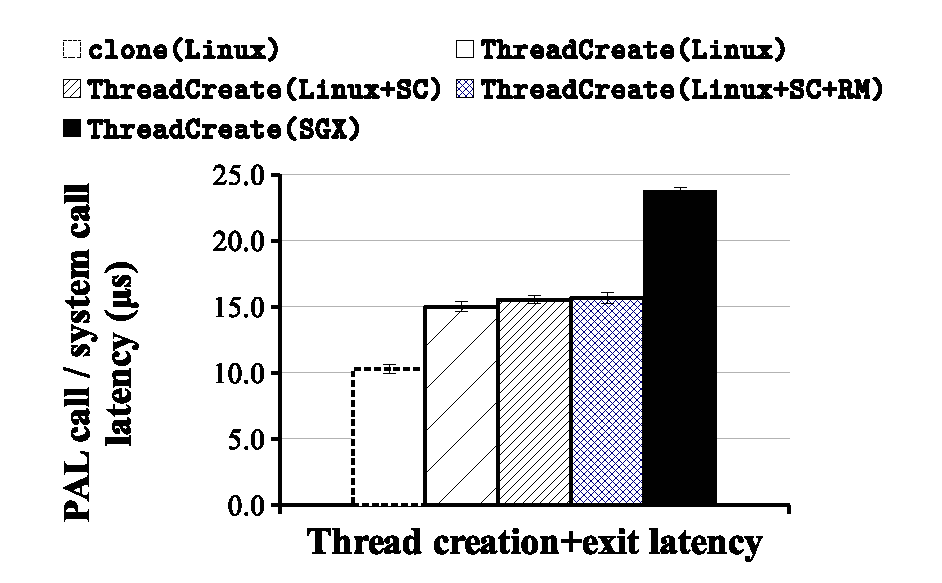
\includegraphics[height=10em]{thread-latency}
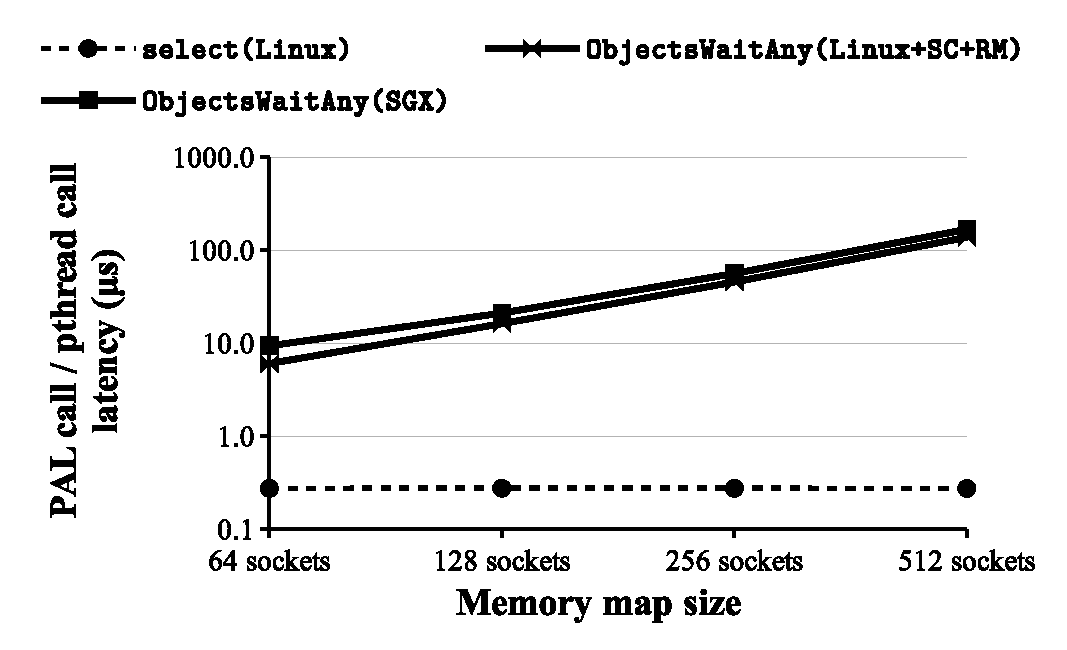
\includegraphics[height=10em]{tcp-select-latency}
}
\parbox{0.49\textwidth}{\centering\bf (a) thread creation}
\parbox{0.49\textwidth}{\centering\bf (b) polling N TCP sockets}
\caption{(a) Thread creation latency and (b) latency of polling a number of TCP sockets.
Lower is better.
The comparison is between (1) \syscall{clone} and \syscall{select} on Linux; (2) \palcall{ThreadCreate} and \palcall{ObjectsWaitAny} on the Linux PAL, with and without a \seccomp{} filter ({\bf +SC}) and reference monitor ({\bf +RM}); (3) the same \hostapis{} on the \sgx{} PAL.}
\label{fig:eval:pal:thread-select-latency}
\end{figure*}


\paragraph{Thread creation.}
Also classified as a single-process operation,
thread creation on Linux PAL
expects little impact from security checks or enforcements.
%which requires no security checks.
%The evaluation shows the latency of creating a new thread within the current process or \picoproc{}.
The implementation effort
for process creation mostly focuses on keeping the semantics of the \hostapi{}---\palcall{ThreadCreate}---as simple as possible.
For instance, a new thread created by \palcall{ThreadCreate} always starts
on a pre-allocated stack
which the guest needs not to assign.
As shown in
Figure~\ref{fig:eval:pal:thread-select-latency} (a),
the overhead
on the Linux PAL
to create and terminate a thread
is \roughly{}46\%,
most of which results from stack allocation.
The overheads of \seccomp{} filter and reference monitor are negligible (less than 5\%).
The latency on the \sgx{} PAL
is slightly more expensive, mostly due to
populating an unused TCS (thread control structure) inside the enclave.
Thread creation on \sgx{} does not accept any inputs
from the untrusted OS,
and thus requires no security checks
against potential Iago attacks.

%The latency of thread creation on the \sgx{} PAL further includes
%the cost of attaching a preallocated enclave thread.
%Inside an enclave,
%the number of concurrent threads is bound by the number
%of TCSes (thread control structure).
%To create a new thread,
%the \sgx{} PAL has to walk the list of TCSes
%to find an unused enclave thread.
%%For the \sgx{} PAL, the cost of thread creation is much higher.
%%Creating an enclave thread on the \sgx{} PAL takes three primary steps: (1) creating an untrusted host thread (a pthread, specifically); (2) attaching the host thread to an unused TCS (thread control section); (3) entering the enclave and initialize its state.
%As a result, the latency of thread creation and exit on the \sgx{} PAL is \roughly{}131\% slower than Linux.




\paragraph{Polling TCP sockets.}
Polling TCP sockets or any stream handles
is one of the operations that suffers more translation costs.
Mapping file, TCP, UDP, or RPC handles
to host file descriptors
requires reading the contents
of handles,
and thus causes overheads
proportional to
numbers of handles.
Figure~\ref{fig:eval:pal:thread-select-latency} (b)
compares the latency of
\palcall{ObjectsWaitAny} on 64 to 512 TCP sockets
with \syscall{select},
and shows that the overhead
of system interface translation is 24--60\% on the Linux PAL.
For the SGX PAL,
polling the same amount
of TCP sockets
requires more time for enclave exits and copying a bitmap of file descriptors
out of the enclave. 
The overhead on the SGX PAL is 13--80\%
compared to \syscall{select}.
%The benchmark result shows that both the Linux and \sgx{} PALs
%have significant overheads
%on polling TCP sockets, at up to 29.1\usec{} and 31.8\usec{}, respectively, for polling 512 sockets.
%The overheads mostly contribute to
%scanning the PAL handle arrays and retrieving
%the file descriptors for polling.
%Although not shown in Figure~\ref{fig:eval:pal:thread-select-latency} (b),
%the overheads
%of the \seccomp{} filter and reference monitor on the Linux PAL
%are negligible.
%The \sgx{} PAL further adds a fixed cost to \palcall{ObjectsWaitAny},
%at \roughly 2.7\usec{},
%for exiting the enclave to poll the file descriptors.





\begin{figure*}[t!]
\centering
\footnotesize
\resizebox{\textwidth}{!}{%
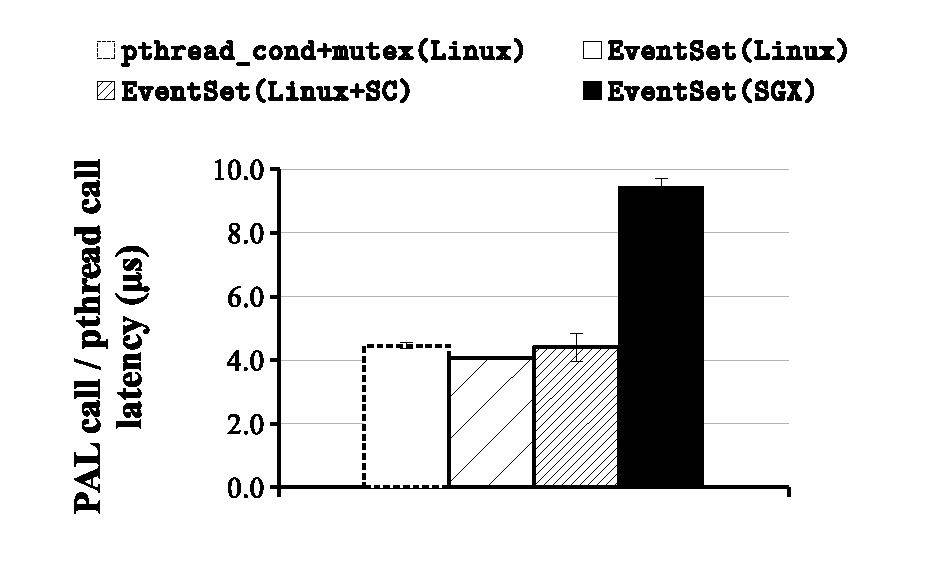
\includegraphics[height=10em]{event-latency}
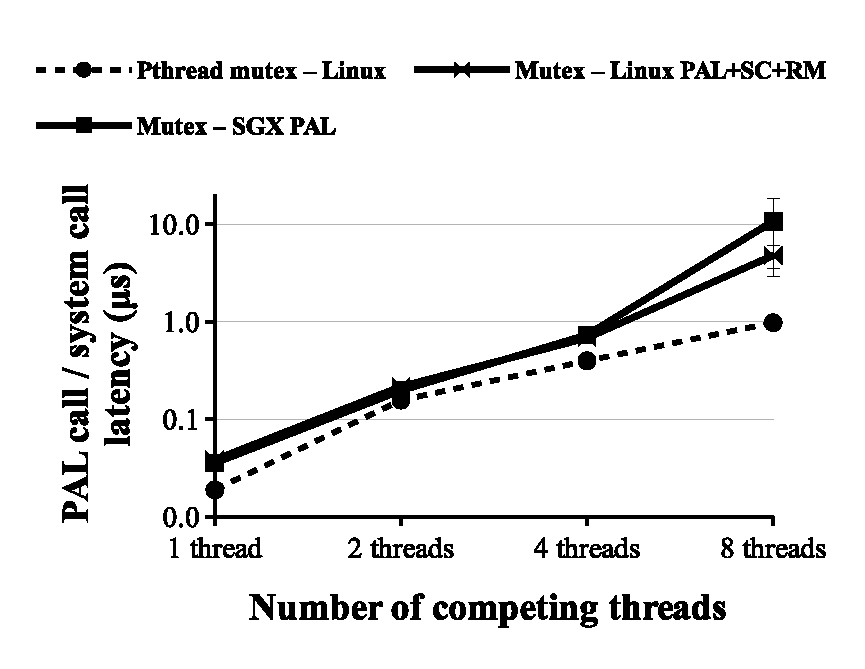
\includegraphics[height=10em]{mutex-latency}
}
\parbox{0.49\textwidth}{\centering\bf (a) signal an event}
\parbox{0.49\textwidth}{\centering\bf (b) competing a mutex among N threads}
\caption{Latency of (a) signaling an event and (b) competing a mutex among N threads (N: 1 to 8).
Lower is better.
The comparison is between (1) pthread condition variables and mutexes on Linux; (2) Notification events and mutexes on the Linux PAL, with and without a \seccomp{} filter ({\bf +SC}) and reference monitor ({\bf +RM}); (3) the same abstractions on the \sgx{} PAL.}
\label{fig:eval:pal:sched-latency}
\end{figure*}




\paragraph{Events and mutexes.}
The Linux PAL and \sgx{} PAL
implement notification events, synchronization events, and mutexes with atomic or compare-and-exchange
instructions,
but use futexes in the host OS
to free the CPUs when blocking on other threads.
The implementation is similar
to pthread primitives such as \code{pthread\_cond} and \code{pthread\_mutex};
therefore, similar performance
is expected on these primitives, with less than 10\% overhead on the Linux PAL.
%Due to the similarity
%of implementation,
%the latency of events and mutexes on the Linux PAL
%are close to
%the corresponding pthread primitives
%(\code{pthread\_cond} and \code{pthread\_mutex}),
%with no more than 10\% overhead 
(see Figure~\ref{fig:eval:pal:sched-latency}).
For the \sgx{} PAL,
these primitives
are much more expensive
(\roughly{}130--250\%)
if the \hostapis{} require exiting enclaves
for futexes.





%Figure~\ref{fig:eval:pal:sched-latency} (a)
%shows the latency of signaling notification events
%on the Linux and \sgx{} PALs.
%For a native Linux process, the pthread library
%provide primitives similar to notification events in \thehostabi{},
%using a combination
%of conditional variables and mutexes.
%In fact, the latency of event signaling on the Linux PAL
%is slightly lower than updating a pthread conditional variable,
%with extra a \roughly{}10\% overhead
%if the \seccomp{} filter and reference monitor is enabled.
%For the \sgx{} PAL, the overhead on signaling an event
%The overhead on the \sgx{} PAL
%is \roughly{}130\%,
%and mostly contributes to the cost of exiting the enclave to call \syscall{futex}.




%The latency of acquiring and releasing a mutex,
%as shown in Figure~\ref{fig:eval:pal:sched-latency} (b),
%is not scalable when multiple threads
%access the same mutex.
%Within a single thread,
%acquiring and releasing a PAL mutex requires no \syscall{futex} calls
%but simply updating a counter
%in the mutex handle.
%If the thread number is increased to two,
%the latency of acquiring and releasing a PAL mutex may still be low
%because
%the Linux PAL always spin for a few rounds to check if
%other thread has released the mutex.
%Afterward, if the mutex is still locked,
%the Linux PAL will block voluntarily,
%by calling \syscall{futex} with \code{FUTEX\_WAIT}.
%With eight threads trying to acquire the same mutex, the latency of acquring and releasing the mutex
%is up to \roughly{}10\usec{}, or 286\% upon the latency of a pthread mutex.
 



